\documentclass[a4paper,11pt]{article}
\usepackage{graphicx}
\usepackage{url}
\usepackage{amsmath}
\usepackage{amsfonts}
\usepackage{geometry}
\usepackage[numbers]{natbib}
\usepackage{cite}
\geometry{margin=1in}
\bibliographystyle{plain}
\graphicspath{{../../04-outputs/01-covid-excess-mortality-replication/}}

\title{Replication Study: Estimating excess mortality in Germany during the COVID-19 pandemic}
\author{}
\date{}

\begin{document}

\maketitle

\section*{Executive Summary}
Germany reported over 150,000 COVID-19 deaths between 2020 and 2023. But what if the real number of lives lost was far higher? By applying a statistical model to pre-pandemic mortality data, we estimate that the country experienced over 240,000 excess deaths\textemdash suggesting that official figures may understate the full impact of the pandemic. This study not only replicates a prominent methodology but also reveals new insights from updated data through 2023. These findings raise critical questions about public health measurement and response strategies.

\section*{Abstract}
We replicate and extend the excess mortality estimation method by Karlinsky and Kobak (2021)\citep{karlinsky2021excess}, applying it to updated German data through 2023. By modeling baseline deaths using 2015–2019 trends, we identify over 240,000 excess deaths during the COVID-19 pandemic. Strikingly, these figures surpass officially reported COVID-19 deaths in every major wave. Our analysis highlights the value of excess mortality as a more comprehensive indicator of pandemic impact\textemdash capturing not only direct fatalities but also those indirectly caused by strained healthcare systems and delayed treatment.

\section{Introduction}
At the heart of any public health crisis lies a fundamental question: how many lives were truly lost? In the case of COVID-19, the answer remains elusive. Official death counts provide a partial picture, constrained by testing availability, shifting reporting standards, and evolving diagnostic criteria. To uncover the pandemic's full impact, researchers increasingly turn to a broader and more robust metric: \emph{excess mortality}\textemdash the number of deaths that exceed the expected baseline in a given period.

This study revisits and extends the method developed by Karlinsky and Kobak (2021)\citep{karlinsky2021excess}, applying it specifically to Germany, a country with one of the most comprehensive and reliable mortality datasets in the world. While the original study focused on early pandemic years, we incorporate updated weekly all-cause mortality data through 2023 and supplement it with COVID-19 death counts from Our World in Data (OWID). This allows us to analyze the full timeline of Germany’s pandemic experience, including recent waves and policy responses.

Beyond replication, our objective is interpretive. We aim to assess the alignment between reported COVID-19 deaths and total excess mortality, identify periods of underestimation, and reflect on what these patterns reveal about health systems, data reliability, and crisis response. In doing so, we move closer to understanding the hidden toll of the pandemic\textemdash not only the deaths that were counted, but also those that were missed.

\section{Data and Methods}

To explore the true scale of pandemic-related mortality in Germany, we adopt a data-driven approach rooted in transparent public datasets and a replicable statistical model. Our analysis is designed to distinguish between officially reported COVID-19 deaths and a broader, more inclusive measure: excess mortality. This section details the data sources, modeling assumptions, and computational strategies we use to quantify and interpret these differences.

\subsection{Data Sources}

We rely on two primary sources of publicly available data:

\begin{itemize}
    \item \textbf{World Mortality Dataset (Karlinsky \& Kobak)}: This dataset provides world weekly counts of all-cause deaths from 2015 through 2023. As one of the most comprehensive international mortality datasets, it forms the backbone of our baseline estimation. By restricting the training period to pre-pandemic years (2015–2019) and the country to Germany, we aim to construct an unbiased reference point for expected deaths.
    
    \item \textbf{Our World in Data (OWID)}: We complement the mortality data with OWID statistics on weekly COVID-19 deaths, vaccination rates, and population figures. These are retrieved as of April 2025 and enable both direct comparison with excess deaths and normalization on a per capita basis.
\end{itemize}

Both datasets are well-maintained and widely used in public health and epidemiological research, making them suitable for a transparent replication study.

\subsection{Statistical Model}

To estimate what mortality would have looked like in the absence of the pandemic, we fit a linear regression model to the 2015–2019 weekly death data. This model includes both long-term trends and seasonal effects:

\[
\mathbb{E}(\text{deaths}_{\text{week}}) = \beta_0 + \beta_1 \cdot \text{year} + \sum_{w=1}^{52} \gamma_w \cdot \text{week}_w
\]

Here, the variable \texttt{year} captures secular time trends (e.g., demographic shifts, improvements in healthcare), while the weekly categorical variables control for seasonal mortality patterns (e.g., winter flu spikes). This modeling choice aligns with the structure introduced in Karlinsky and Kobak (2021), allowing for comparability while maintaining simplicity and interpretability.

\subsection{Excess Mortality and P-score}

Once the expected weekly deaths are modeled, excess mortality is defined as the difference between observed and expected values:

\[
\text{Excess Deaths}_{t} = \text{Observed Deaths}_{t} - \text{Expected Deaths}_{t}
\]

To contextualize the magnitude of these deviations, we compute the P-score, which expresses excess mortality as a percentage of the baseline:

\[
\text{P-score}_{t} = 100 \times \frac{\text{Excess Deaths}_{t}}{\text{Expected Deaths}_{t}}
\]

P-scores allow us to compare different periods and countries on a normalized scale, revealing when and where mortality anomalies occurred most acutely. A P-score of 40\% implies that deaths in that week were 40\% higher than expected, regardless of population size.

\subsection{Comparing with Reported COVID-19 Deaths}

To evaluate potential underreporting or indirect mortality, we compare weekly excess deaths with officially reported COVID-19 deaths from OWID. Recognizing that population growth may influence raw numbers, we normalize both metrics per 100,000 people using weekly population estimates. This allows for meaningful per capita comparisons and helps disentangle demographic effects from mortality trends.

Importantly, this comparative lens offers insights into when and where reported COVID-19 deaths may have significantly underestimated the broader human toll\textemdash either due to testing limitations, classification gaps, or indirect consequences such as delayed treatment and reduced healthcare access.

\section{Results}

\subsection{Observed vs. Expected Deaths}

\begin{figure}[h]
\centering
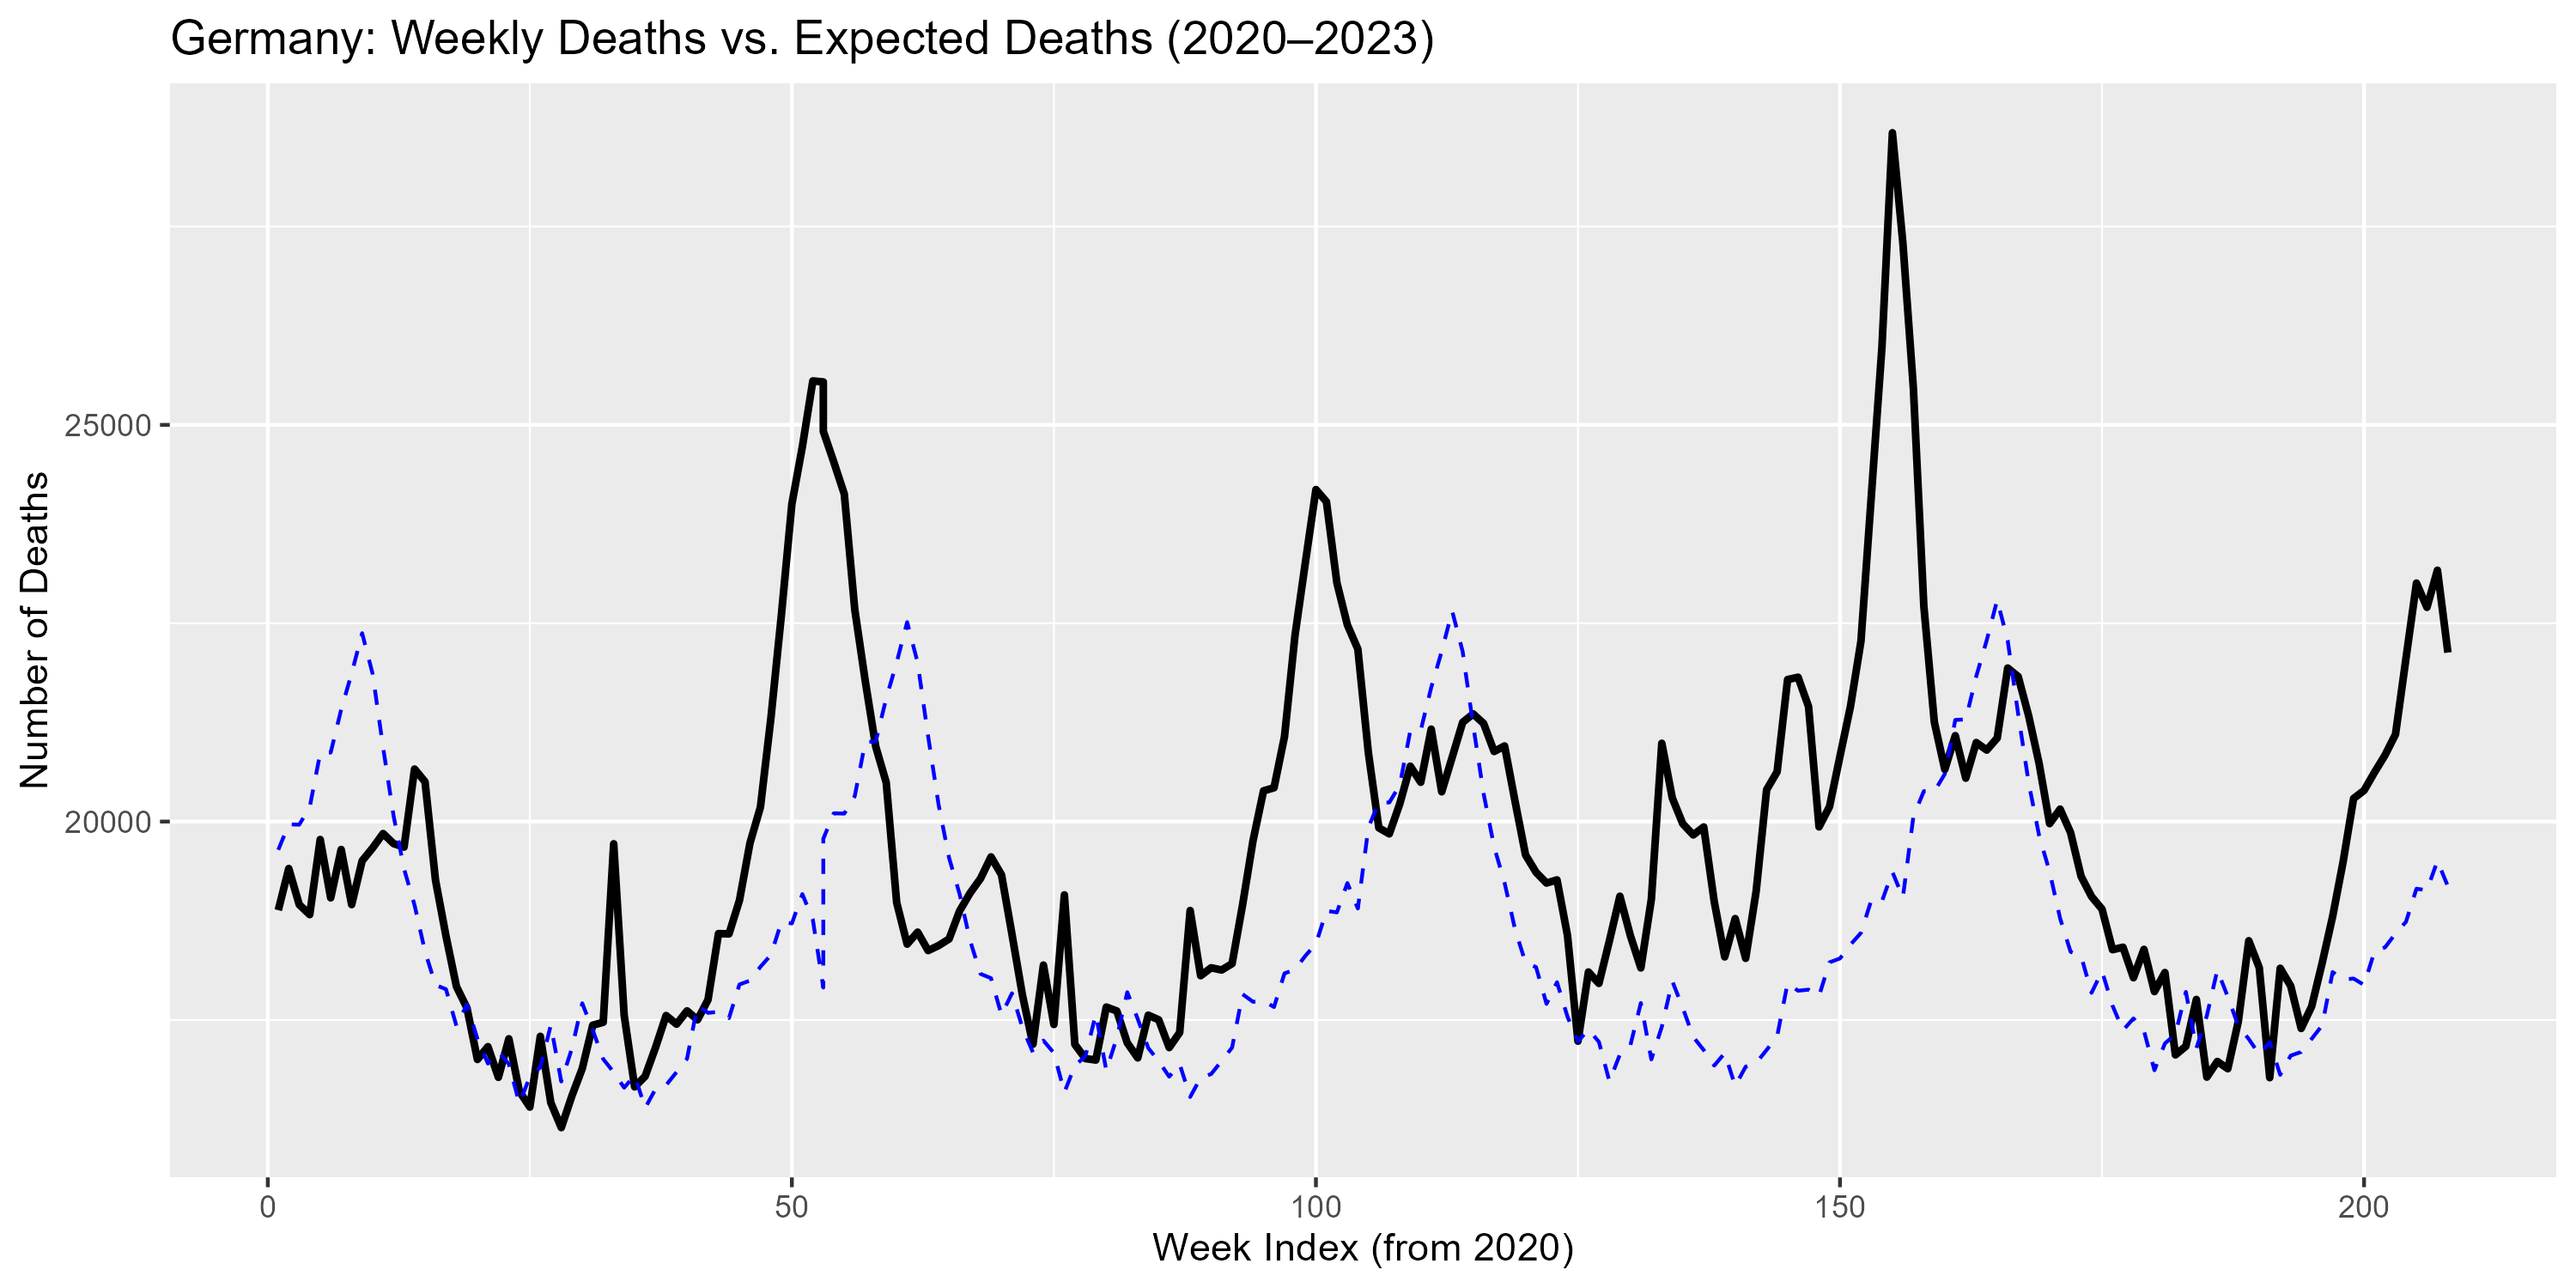
\includegraphics[width=0.9\textwidth]{Figure1-germany-deaths-vs-expected.png}
\caption{Germany weekly observed vs. expected deaths (2020–2023).}\label{f1}
\end{figure}

Figure \ref{f1} illustrates the divergence between actual and expected mortality across the four years of the pandemic. Each winter season reveals a pronounced spike in observed deaths, significantly surpassing the modeled baseline. These patterns strongly align with the known timing of COVID-19 surges in Germany. Even during certain spring and summer periods, smaller waves of excess mortality are visible, indicating that the impact of the pandemic was not confined to traditional flu seasons. The overall alignment between observed death peaks and known viral transmission waves strengthens confidence in the model’s relevance.

\subsection{Excess Deaths and P-scores}

\begin{figure}[h]
\centering
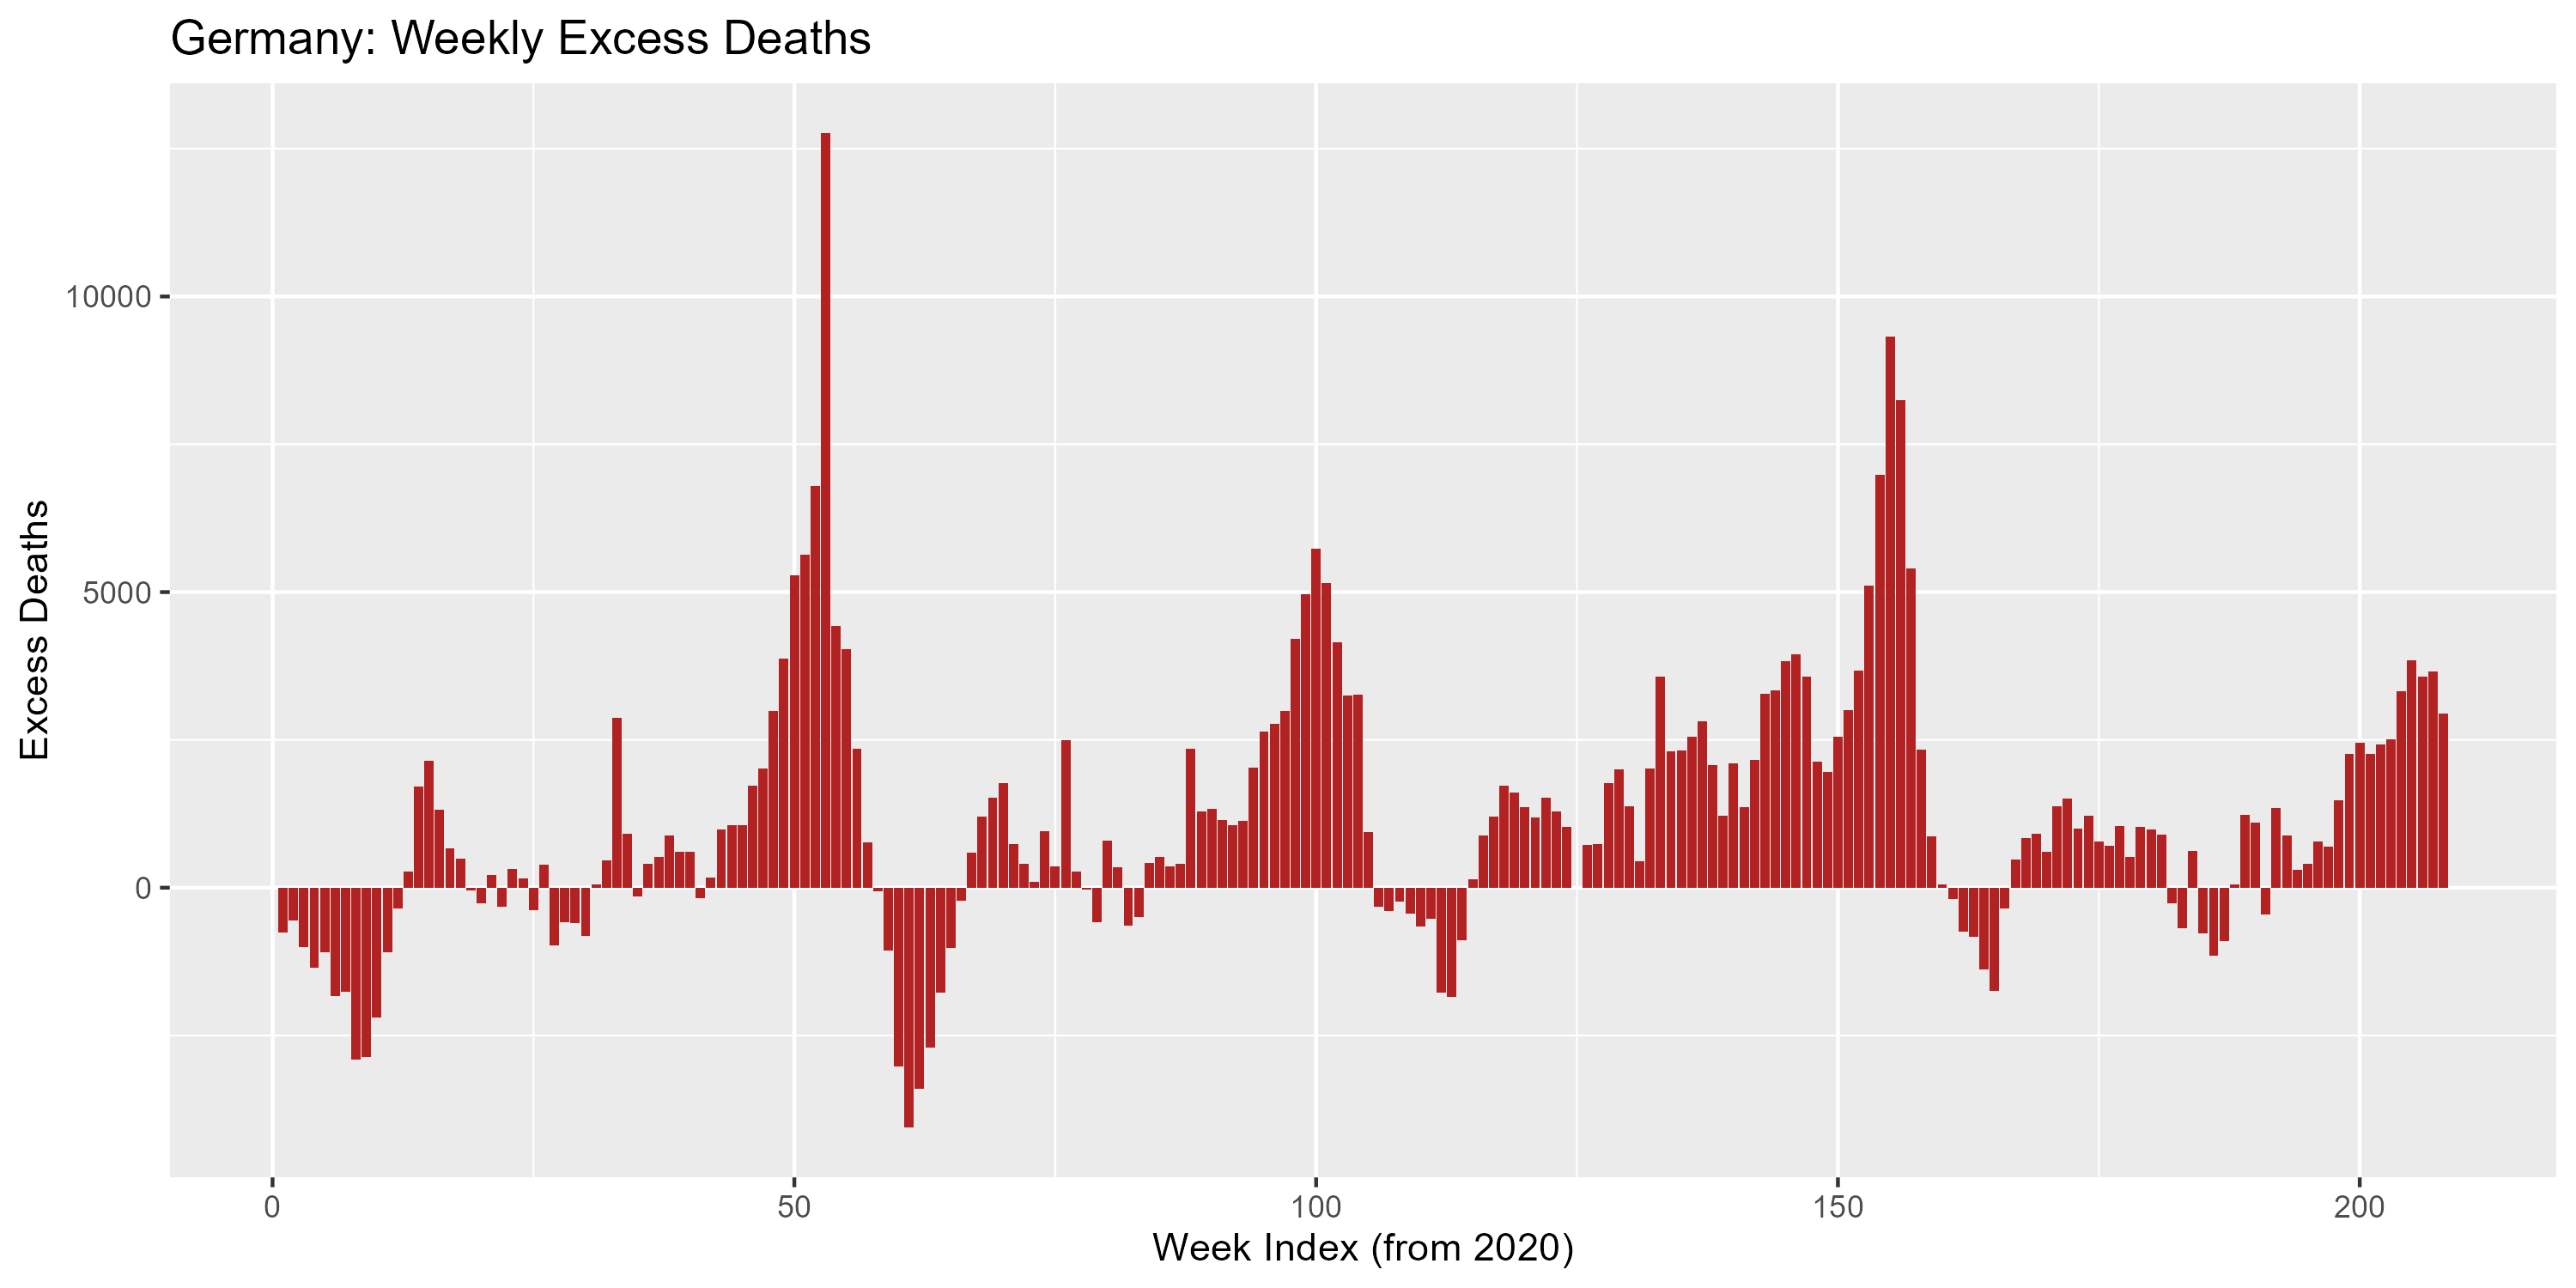
\includegraphics[width=0.9\textwidth]{Figure2-germany-excess-deaths.png}
\caption{Weekly excess deaths.}\label{f2}
\end{figure}

\begin{figure}[h]
\centering
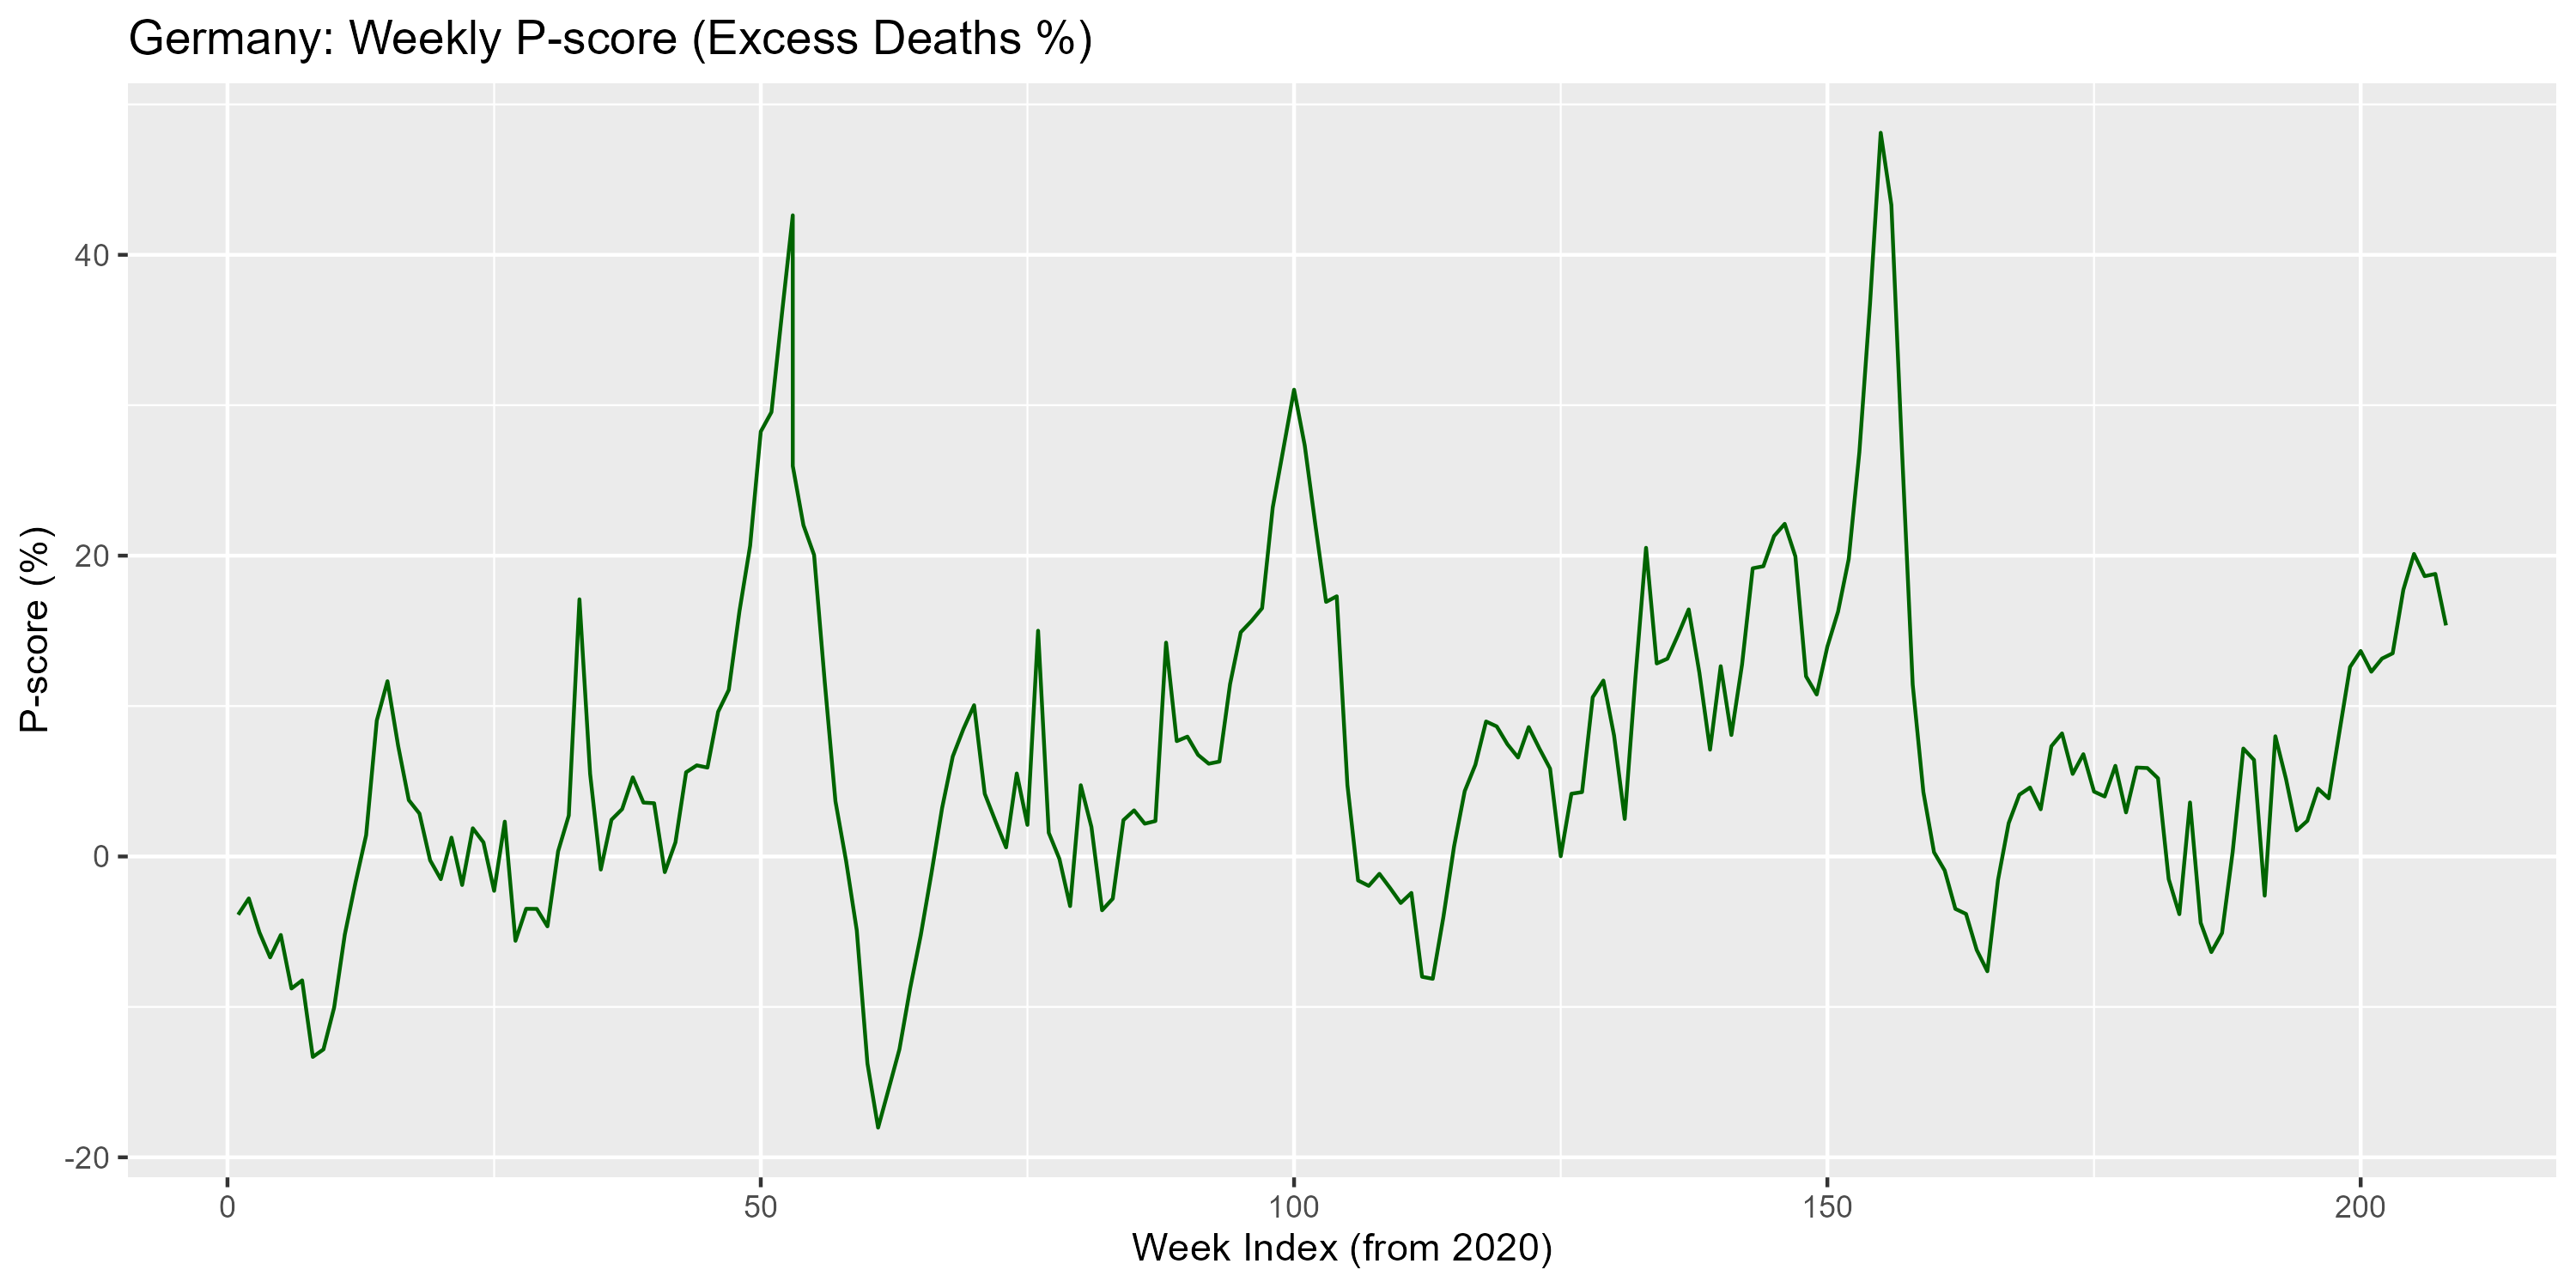
\includegraphics[width=0.9\textwidth]{Figure3-germany-p-score.png}
\caption{P-score: Percentage above baseline.}\label{f3}
\end{figure}

Figures \ref{f2} and \ref{f3} present excess deaths in absolute numbers and relative percentages (P-scores), respectively. In several winter weeks\textemdash particularly during early 2021 and late 2022\textemdash excess deaths surpassed 10,000 per week, pointing to extreme pressure on the healthcare system and potentially underreported COVID-19 fatalities. The P-score plot further contextualizes these events: at their peaks, mortality rates exceeded the expected baseline by over 40\%. Such deviations cannot be explained by typical seasonal variation alone and underscore the pandemic’s profound disruption of normal mortality patterns.

\subsection{Reported COVID-19 vs Excess Mortality}

\begin{figure}[h]
\centering
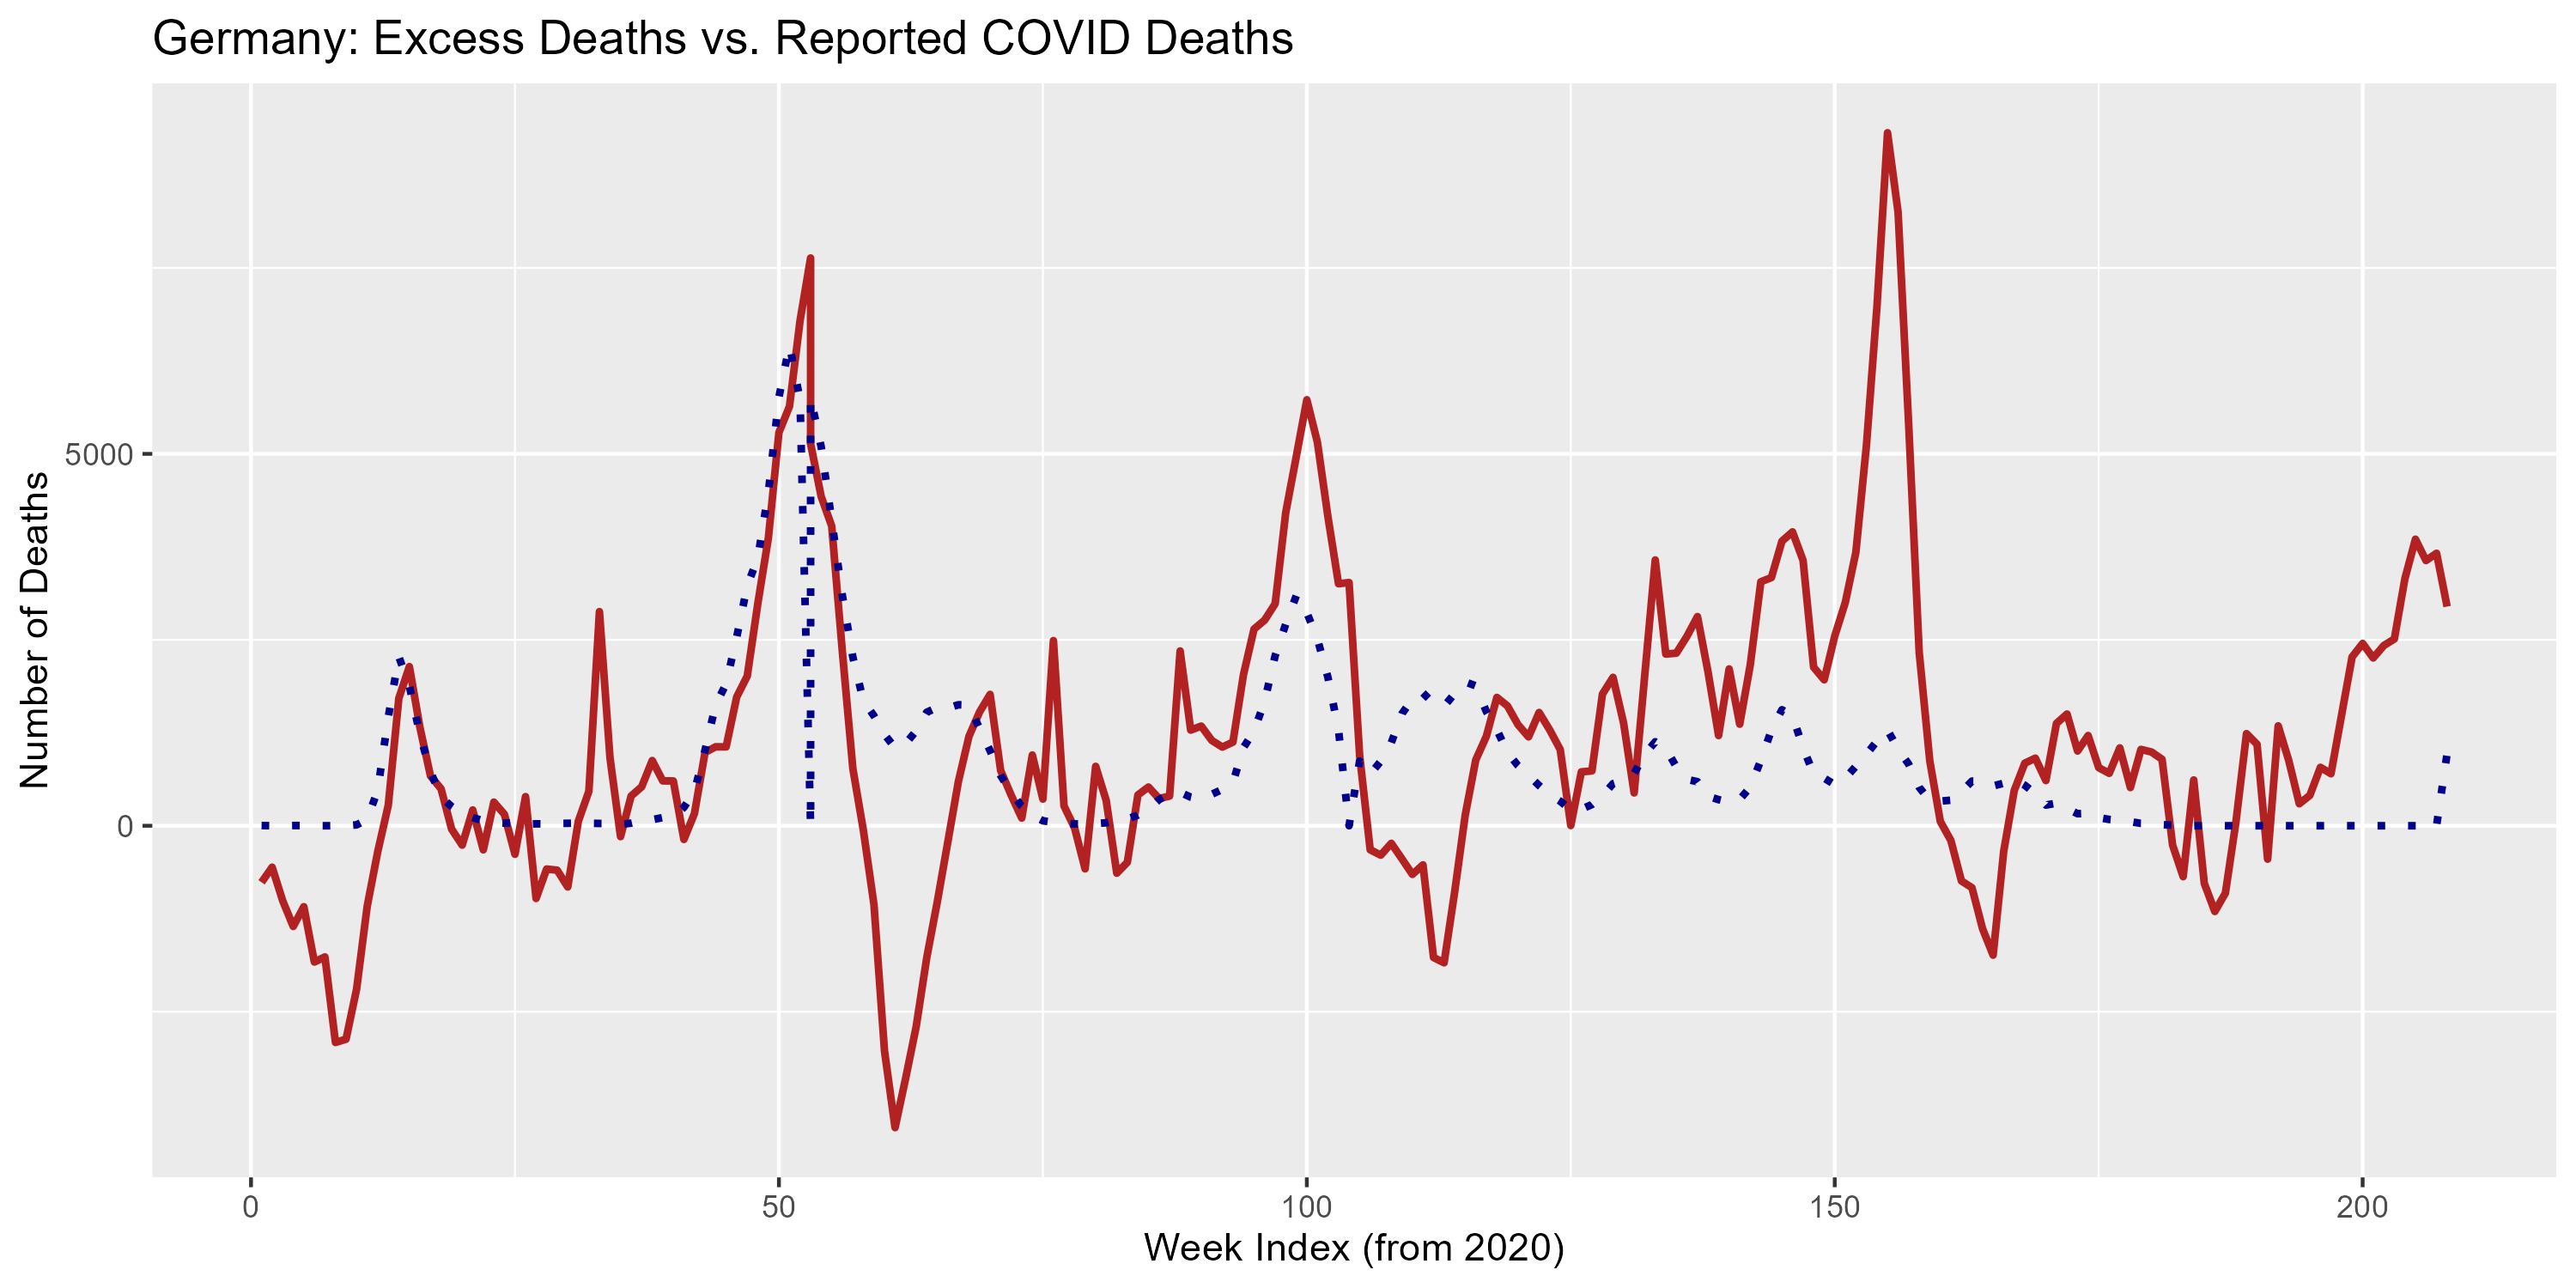
\includegraphics[width=0.9\textwidth]{Figure4-germany-excess-vs-covid.png}
\caption{Excess deaths (line) vs reported COVID-19 deaths (dotted).}\label{f4}
\end{figure}

Figure \ref{f4} compares weekly excess deaths with officially reported COVID-19 deaths. A consistent pattern emerges: excess mortality often exceeds the number of deaths attributed to COVID-19, especially during major peaks. The most striking discrepancy appears in 2022, when excess deaths surged while official COVID-19 counts remained relatively subdued. This suggests that a significant portion of pandemic-related deaths may have been misclassified or indirectly caused by broader disruptions\textemdash such as delayed access to care, economic hardship, or mental health deterioration. The visual gap between the two curves reinforces the argument that excess mortality captures a broader and more inclusive picture of the pandemic’s human toll.

\subsection{Summary Statistics}

\begin{center}
\begin{tabular}{|c|c|c|c|}
\hline
\textbf{Year} & \textbf{Excess Deaths} & \textbf{Peak P-score (\%)} & \textbf{Reported COVID-19 Deaths} \\
\hline
2020 & 32,135 & 42.6 & 47,009 \\
2021 & 60,386 & 31.0 & 64,939 \\
2022 & 98,320 & 48.1 & 48,046 \\
2023 & 51,243 & 26.9 & 9,241 \\
\hline
\end{tabular}
\end{center}

These figures reinforce the narrative seen in the visualizations. In every year of the pandemic, excess deaths either matched or exceeded officially reported COVID-19 deaths\textemdash with the most dramatic mismatch in 2022, when nearly 100,000 excess deaths were recorded compared to just over 48,000 COVID-19 deaths. Even in 2023, with vaccination rates high and pandemic restrictions eased, the excess death count remained disproportionately elevated relative to reported COVID-19 fatalities. These patterns call attention to uncounted losses and compel closer scrutiny of both public health reporting systems and indirect pandemic effects.

\section{Discussion}

This analysis reveals significant divergence between officially reported COVID-19 deaths and the broader pattern of excess mortality in Germany between 2020 and 2023. Across multiple waves of the pandemic, weekly deaths consistently exceeded modelled expectations, suggesting that the crisis had deeper and more widespread effects than captured by direct attribution alone. Notably, 2022 emerged as a particularly anomalous year, with excess deaths far outpacing reported COVID-19 fatalities\textemdash an indication that indirect effects may have intensified over time.

Several possible explanations arise from this discrepancy. Early limitations in diagnostic capacity, inconsistent death certification, and evolving testing protocols may have contributed to initial undercounting. Over time, the indirect consequences of prolonged health system strain likely became more pronounced. Factors such as postponed surgeries, reduced access to routine care, increased mental health burden, and socioeconomic disruptions could have led to preventable mortality unrelated to the virus itself.

These findings speak to a broader challenge in health surveillance: even in high-capacity systems like Germany's, gaps persist in the timely and accurate recording of public health outcomes. This raises concerns about the reliability of pandemic monitoring globally, especially in lower-resource settings where data quality may be weaker. In that context, excess mortality serves as a crucial aggregate indicator, capturing effects that elude traditional case- or cause-based reporting.

That said, limitations in our approach warrant careful interpretation. The model does not incorporate dynamic population changes, such as aging or migration, and it treats each week independently, without modeling long-term structural shifts. Nor does excess mortality analysis allow for precise attribution of causes\textemdash making it difficult to disentangle deaths from COVID-19 versus those caused by policy fallout, deferred care, or unrelated events. Addressing these issues requires more granular demographic and cause-of-death data, alongside multidisciplinary collaboration in future work.

\section{Conclusion}

This study extends prior work on pandemic mortality estimation by applying a validated excess mortality framework to updated data from Germany through the end of 2023. By comparing observed deaths to a counterfactual baseline derived from pre-pandemic years, we estimate that Germany experienced over 240,000 excess deaths during the pandemic\textemdash far exceeding officially reported COVID-19 fatalities in several periods.

These findings highlight the limitations of relying solely on confirmed case and death counts to assess the impact of a public health crisis. While useful for real-time response, official tallies often fail to capture the broader ripple effects of systemic disruption. Excess mortality, in contrast, reflects a more comprehensive view, integrating both direct viral mortality and indirect consequences, such as delayed treatment or increased social vulnerability.

Looking forward, there is clear value in strengthening national mortality tracking systems with demographic, geographic, and clinical specificity. Incorporating regional variations, age structures, and detailed cause-of-death categories would enable more accurate identification of both vulnerable populations and systemic weak points. At the same time, future studies could benefit from linking excess mortality with contextual variables such as healthcare capacity, public policy timing, and behavioral responses.

Ultimately, capturing the full toll of a pandemic requires more than counting infections or attributing causes. It demands a holistic framework that reflects the cascading effects of crisis on health, infrastructure, and society. This analysis contributes to that broader understanding and provides a foundation for more resilient health surveillance moving forward.

\bibliography{bibliography}

\end{document}
